%%%%%%%%%%%%%%%%%%%%%%%%%%%%%%%%%%%%%%%%%%%%%%%%%%%%%%%%%%%%%%%%%%%%%%%%%%%
%% This file is part of the book
%%
%% Algorithmic Graph Theory
%% http://code.google.com/p/graph-theory-algorithms-book/
%%
%% Copyright (C) 2010 David Joyner <wdjoyner@gmail.com>
%% Copyright (C) 2009, 2010, 2011 Minh Van Nguyen <nguyenminh2@gmail.com>
%%
%% See the file COPYING for copying conditions.
%%%%%%%%%%%%%%%%%%%%%%%%%%%%%%%%%%%%%%%%%%%%%%%%%%%%%%%%%%%%%%%%%%%%%%%%%%%

\chapter{Distance and Connectivity}
\label{chap:distance_connectivity}

\begin{quote}
\footnotesize
\index{biology}
\index{chemistry}
\index{social network}
\includegraphics[scale=0.85]{image/distance-connectivity/what-is-math} \\
\noindent
--- Spiked Math,
\url{http://spikedmath.com/382.html}
\end{quote}


%%%%%%%%%%%%%%%%%%%%%%%%%%%%%%%%%%%%%%%%%%%%%%%%%%%%%%%%%%%%%%%%%%%%%%%%%%%

\section{Paths and distance}


%%%%%%%%%%%%%%%%%%%%%%%%%%%%%%%%%%%%%%%%%%%%%%%%%%%%%%%%%%%%%%%%%%%%%%%%%%%

\subsection{Distance and metrics}

Consider an edge-weighted simple graph $G = (V,E,i,h)$ without
negative weight cycles. Here $E \subseteq V^{(2)}$, $i: E \to V^{(2)}$
is an incidence function as in~\eqref{eqn:introduction:edge_incidence},
which we regard as the identity function, and $h: E \to V$ is an
orientation function as in~\eqref{eqn:introduction:edge_orientation}.
Let $W: E \to \R$ be the weight function. (If $G$ is not provided with
a weight function on the edges, we assume that each edge has unit
weight.) If $v_1, v_2 \in V$ are two vertices and
$P = (e_1, e_2, \dots, e_m)$ is a $v_1$-$v_2$ path~(so $v_1$ is
incident to $e_1$ and $v_2$ is incident to $e_m$), define the
\emph{weight}\index{weight!path} of $P$ to be the sum of the weights
of the edges in $P$:
\[
W(P)
=
\sum_{i=1}^m W(e_i).
\]
The \emph{distance function}\index{distance!function}
$d: V \times V \to \R \cup \{\infty\}$ on $G$ is defined by
\[
d(v_1, v_2)
=
\infty
\]
if $v_1$ and $v_2$ lie in distinct connected components of $G$, and by
%%
\begin{equation}
\label{eqn:distance_connectivity:distance_as_minimum_path_weight}
d(v_1, v_2)
=
\min_P W(P)
\end{equation}
%%
otherwise, where the minimum is taken over all paths $P$ from $v_1$ to
$v_2$. By hypothesis, $G$ has no negative weight cycles so the minimum
in~\eqref{eqn:distance_connectivity:distance_as_minimum_path_weight}
exists. It follows by definition of the distance function that
$d(u,v) = \infty$ if and only if there is no path between $u$ and $v$.

How we interpret the distance function $d$ depends on the meaning of
the weight function $W$. In practical applications, vertices can
represent physical locations such as cities, sea ports, or
landmarks. An edge weight could be interpreted as the physical
distance in kilometers between two cities, the monetary cost of
shipping goods from one sea port to another, or the time required to
travel from one landmark to another. Then $d(u,v)$ could mean the
shortest route in kilometers between two cities, the lowest cost
incurred in transporting goods from one sea port to another, or the
least time required to travel from one landmark to another.

The distance function\index{distance!function} $d$ is not in general a
metric\index{metric}, i.e. the triangle
inequality\index{triangle inequality} does not in general hold for
$d$. However, when the distance function is a metric then $G$ is
called a \emph{metric graph}\index{metric graph}. The theory of
metric\index{metric graph} graphs, due to their close connection with
tropical curves, is an active area of research. For more information
on metric graphs, see Baker\index{Baker, Matthew} and
Faber\index{Faber, Xander}~\cite{BakerFaber2006}.


%%%%%%%%%%%%%%%%%%%%%%%%%%%%%%%%%%%%%%%%%%%%%%%%%%%%%%%%%%%%%%%%%%%%%%%%%%%

\subsection{Radius and diameter}

A new hospital is to be built in a large city. Construction has not
yet started and a number of urban planners are discussing the future
location of the new hospital. What is a possible location for the new
hospital and how are we to determine this location? This is an example
of a class of problems known as facility location problems. Suppose
our objective in selecting a location for the hospital is to minimize
the maximum response time between the new hospital and the site of an
emergency. To help with our decision making, we could use the notion
of the center of a graph.

The center of a graph $G = (V,E)$ is defined in terms of the
eccentricity of the graph under consideration. The
\emph{eccentricity}\index{eccentricity}
$\epsilon: V \to \R$\index{$\epsilon$} is defined as follows. For any
vertex $v$, the eccentricity $\epsilon(v)$ is the greatest distance
between $v$ and any other vertex in $G$. In symbols, the eccentricity
is expressible as
\[
\epsilon(v)
=
\max_{u \in V} d(u,v).
\]
For example, in a tree $T$ with root $r$ the eccentricity of $r$ is
the height of $T$. In the graph of
Figure~\ref{fig:distance_connectivity:find_eccentricity_center_radius_diameter},
the eccentricity of $2$ is $5$ and the shortest paths that yield
$\epsilon(2)$ are
%%
\begin{align*}
P_1: 2, 3, 4, 14, 15, 16 \\
P_2: 2, 3, 4, 14, 15, 17.
\end{align*}
%%
The eccentricity of a vertex $v$ can be thought of as an upper bound
on the distance from $v$ to any other vertex in $G$. Furthermore, we
have at least one vertex in $G$ whose distance from $v$ is
$\epsilon(v)$.

\begin{figure}[!htbp]
\centering
\includegraphics{image/distance-connectivity/determine-eccentricity-radius-diameter}
\caption{Determine the eccentricity, center, radius, and diameter.}
\label{fig:distance_connectivity:find_eccentricity_center_radius_diameter}
\end{figure}

\begin{table}[!htbp]
\centering
\index{eccentricity}
%%%%%%%%%%%%%%%%%%%%%%%%%%%%%%%%%%%%%%%%%%%%%%%%%%%%%%%%%%%%%%%%%%%%%%%%%%%
%% This file is part of the book
%%
%% Algorithmic Graph Theory
%% http://code.google.com/p/graph-theory-algorithms-book/
%%
%% Copyright (C) 2009--2011 Minh Van Nguyen <nguyenminh2@gmail.com>
%%
%% See the file COPYING for copying conditions.
%%%%%%%%%%%%%%%%%%%%%%%%%%%%%%%%%%%%%%%%%%%%%%%%%%%%%%%%%%%%%%%%%%%%%%%%%%%

\begin{tabular}{r|ccccccccccccccccc}
$v$ & $1$ & $2$ & $3$ & $4$ & $5$ & $6$ & $7$ & $8$ & $9$ & $10$ & $11$ & $12$ & $13$ & $14$ & $15$ & $16$ & $17$ \\\hline
$\epsilon(v)$ & $6$ & $5$ & $4$ & $4$ & $5$ & $6$ & $7$ & $7$ & $5$ & $6$ & $7$ & $7$ & $6$ & $5$ & $6$ & $7$ & $7$
\end{tabular}

\caption{Eccentricity distribution for the graph in
  Figure~\ref{fig:distance_connectivity:find_eccentricity_center_radius_diameter}.}
\label{tab:distance_connectivity:eccentricity_distribution}
\end{table}

\begin{figure}[!htbp]
\centering
\index{eccentricity}
\includegraphics{image/distance-connectivity/eccentricity-distribution}
\caption{Eccentricity distribution of the graph in
  Figure~\ref{fig:distance_connectivity:find_eccentricity_center_radius_diameter}.
  The horizontal axis represents the vertex name, while the vertical
  axis is the corresponding eccentricity.}
\label{fig:distance_connectivity:eccentricity_distribution}
\end{figure}

To motivate the notion of the radius of a graph, consider the
distribution of eccentricity among vertices of the graph $G$ in
Figure~\ref{fig:distance_connectivity:find_eccentricity_center_radius_diameter}.
The required eccentricity distribution is shown in
Table~\ref{tab:distance_connectivity:eccentricity_distribution}. Among
the eccentricities in the latter table, the minimum eccentricity is
$\epsilon(3) = \epsilon(4) = 4$. An intuitive interpretation is that
both of the vertices $3$ and $4$ have the shortest distance to any
other vertices in $G$. We can invoke an analogy with plane geometry as
follows. If a circle has radius $r$, then the distance from the center
of the circle to any point within the circle is at most $r$. The
minimum eccentricity in graph theory plays a role similar to the
radius of a circle. If an object is strategically
positioned---e.g. a vertex with minimum eccentricity or the center of
a circle---then its greatest distance to any other object is
guaranteed to be minimum. With the above analogy in mind, we define
the \emph{radius} of a graph $G = (V,E)$, written
$\radius(G)$\index{$\radius(G)$}, to be the minimum eccentricity among
the eccentricity distribution of $G$. In symbols,
\[
\radius(G)
=
\min_{v \in V} \epsilon(v).
\]
The \emph{center} of $G$, written $C(G)$, is the set of vertices with
minimum eccentricity. Thus the graph in
Figure~\ref{fig:distance_connectivity:find_eccentricity_center_radius_diameter}
has radius $4$ and center $\{3, 4\}$. As should be clear from the
latter example, the radius is a number whereas the center is a
set. Refer to the beginning of the section where we mentioned the
problem of selecting a location for a new hospital. We could use a
graph to represent the geography of the city wherein the hospital is
to be situated and select a location that is in the center of the
graph.

Consider now the maximum eccentricity of a
graph. In~\eqref{eqn:graph_algorithms:graph_diameter} we defined the
\emph{diameter} of a graph $G = (V,E)$ by
\[
\diam(G)\index{$\diam(G)$}
=
\max_{\substack{u,v \in V \\ u \neq v}} d(u,v).
\]
The diameter of $G$ can also be defined as the maximum eccentricity of
any vertex in $G$:
\[
\diam(G)
=
\max_{v \in V} \epsilon(v).
\]
In case $G$ is disconnected, define its diameter to be
$\diam(G) = \infty$. To compute $\diam(G)$, use the Floyd-Roy-Warshall
algorithm~(see
section~\ref{sec:graph_algorithms:Floyd_Roy_Warshall_algorithm}) to
compute the shortest distance between each pair of vertices. The
maximum of these distances is the diameter. The set of vertices of $G$
with maximum eccentricity is called the \emph{periphery} of $G$,
written $\per(G)$\index{$\per(G)$}. The graph in
Figure~\ref{fig:distance_connectivity:find_eccentricity_center_radius_diameter}
has diameter $7$ and periphery $\{7, 8, 11, 12, 16, 17\}$.

\begin{theorem}
\textbf{Eccentricities of adjacent vertices.}
Let $G = (V,E)$ be an undirected, connected graph having nonnegative
edge weights. If $uv \in E$ and $W$ is a weight function for $G$, then
$|\epsilon(u) - \epsilon(v)| \leq W(uv)$.
\end{theorem}

\begin{proof}
By definition, we have $d(u,x) \leq \epsilon(u)$ and
$d(v,x) \leq \epsilon(v)$ for all $x \in V$. Let $w \in V$ such that
$d(u,w) = \epsilon(u)$. Apply the triangle inequality to obtain
%%
\begin{align*}
d(u,w) &\leq d(u,v) + d(v,w) \\
\epsilon(u) &\leq W(uv) + d(v,w) \\
            &\leq W(uv) + \epsilon(v)
\end{align*}
%%
from which we have $\epsilon(u) - \epsilon(v) \leq W(uv)$. Repeating
the above argument with the role of $u$ and $v$ interchanged yields
$\epsilon(v) - \epsilon(u) \leq W(uv)$. Both
$\epsilon(u) - \epsilon(v) \leq W(uv)$ and
$\epsilon(v) - \epsilon(u) \leq W(uv)$ together yields the inequality
$|\epsilon(u) - \epsilon(v)| \leq W(uv)$ as required.
\end{proof}


%%%%%%%%%%%%%%%%%%%%%%%%%%%%%%%%%%%%%%%%%%%%%%%%%%%%%%%%%%%%%%%%%%%%%%%%%%%

\subsection{Center of trees}

Given a tree $T$ of order $\geq 3$, we want to derive a bound on the
number of vertices that comprise the center of $T$. A graph in general
can have one, two, or more number of vertices for its center. Indeed,
for any integer $n > 0$ we can construct a graph whose center has
cardinality $n$. The cases for $n = 1, 2, 3$ are illustrated in
Figure~\ref{fig:distance_connectivity:graphs_arbitrarily_large_centers}. But
can we do the same for trees? That is, given any positive integer $n$
does there exist a tree whose center has $n$ vertices? It turns out
that the center of a tree cannot have more than two vertices, a result
first discovered~\cite{Jordan1869} by Camille
Jordan\index{Jordan, Camille} in~1869.

\begin{figure}[!htbp]
\centering
%%%%%%%%%%%%%%%%%%%%%%%%%%%%%%%%%%%%%%%%%%%%%%%%%%%%%%%%%%%%%%%%%%%%%%%%%%%
%% This file is part of the book
%%
%% Algorithmic Graph Theory
%% http://code.google.com/p/graph-theory-algorithms-book/
%%
%% Copyright (C) 2009, 2010, 2011 Minh Van Nguyen <nguyenminh2@gmail.com>
%%
%% See the file COPYING for copying conditions.
%%%%%%%%%%%%%%%%%%%%%%%%%%%%%%%%%%%%%%%%%%%%%%%%%%%%%%%%%%%%%%%%%%%%%%%%%%%

\documentclass{article}

\usepackage{subfigure}
\usepackage{tikz}
\usetikzlibrary{external}
\tikzexternalize{arbitrarily-large-center}

\begin{document}

\begin{figure}
\subfigure[$|C(G)| = 1$]{
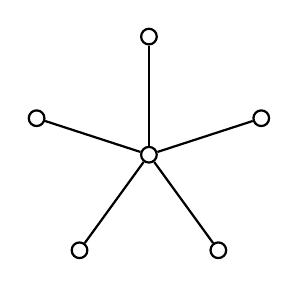
\begin{tikzpicture}
[nodeDecorate/.style={shape=circle,inner sep=2pt,draw,thick},%
  lineDecorate/.style={-,thick},%
  scale=1.5]
%% complete bipartite graph K_{1,5}
%% nodes or vertices
\foreach \nodename/\x/\y in {
  1/0.9510/0.3090, 2/0/1, 3/-0.9510/0.3090, 4/-0.5877/-0.8090,
  5/0.5877/-0.8090, 6/0/0}
{
  \node (\nodename) at (\x,\y) [nodeDecorate] {};
}
%% edges or lines
\path
\foreach \startnode/\endnode in {1/6, 2/6, 3/6, 4/6, 5/6}
{
  (\startnode) edge[lineDecorate] node {} (\endnode)
};
\end{tikzpicture}
}
%%
%%
\qquad
\subfigure[$|C(G)| = 2$]{
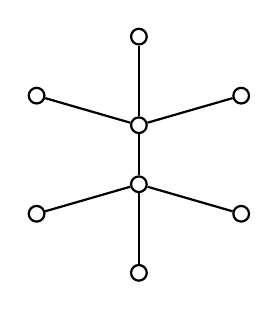
\begin{tikzpicture}
[nodedecorate/.style={shape=circle,inner sep=2pt,draw,thick},%
  linedecorate/.style={-,thick},%
  scale=1.5]
%% nodes or vertices
\foreach \nodename/\x/\y in {1/0.8660/0.5, 2/0/1, 3/-0.8660/0.5,
  4/-0.8660/-0.5, 5/0/-1, 6/0.8660/-0.5, 7/0/0.25, 8/0/-0.25}
{
  \node (\nodename) at (\x,\y) [nodedecorate] {};
}
%% edges or lines
\path
\foreach \startnode/\endnode in {7/1, 7/2, 7/3, 7/8, 8/4, 8/5, 8/6}
{
  (\startnode) edge[linedecorate] node {} (\endnode)
};
\end{tikzpicture}
}
%%
%%
\qquad
\subfigure[$|C(G)| = 3$]{
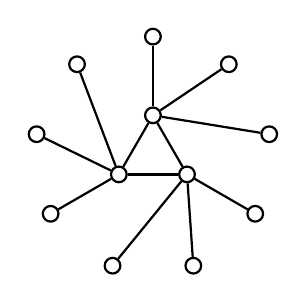
\begin{tikzpicture}
[nodedecorate/.style={shape=circle,inner sep=2pt,draw,thick},%
  linedecorate/.style={-,thick},%
  scale=1.5]
%% nodes or vertices
\foreach \nodename/\x/\y in {
  %% outer vertices
  1/0/1, 2/0.6427/0.7660, 3/0.9848/0.1736, 4/0.8660/-0.5,
  5/0.3420/-0.9396, 6/-0.3420/-0.9396, 7/-0.8660/-0.5,
  8/-0.9848/0.1736, 9/-0.6427/0.7660,
  %% inner vertices
  10/0/0.3333, 11/0.2886/-0.1666, 12/-0.2886/-0.1666}
{
  \node (\nodename) at (\x,\y) [nodedecorate] {};
}
%% edges or lines
\path
\foreach \startnode/\endnode in {
  10/1, 10/2, 10/3, 11/4, 11/5, 11/6, 12/7, 12/8, 12/9, 10/11, 11/12, 12/10}
{
  (\startnode) edge[linedecorate] node {} (\endnode)
};
\end{tikzpicture}
}
\end{figure}

\end{document}

\caption{Constructing graphs with arbitrarily large centers.}
\label{fig:distance_connectivity:graphs_arbitrarily_large_centers}
\end{figure}

\begin{theorem}
\textbf{Jordan~\cite{Jordan1869}.}
If a tree $T$ has order $\geq 3$, then the center of $T$ is either a
single vertex or two adjacent vertices.
\end{theorem}

\begin{proof}
As all eccentric vertices of $T$ are leaves~(see
problem~\ref{chap:distance_connectivity}.\ref{prob:distance_connectivity:eccentric_vertices_laves}),
removing all the leaves of $T$ decreases the eccentricities of the
remaining vertices by one. The tree comprised of the surviving
vertices has the same center as $T$. Continue pruning leaves as
described above and note that the tree comprised of the surviving
vertices has the same center as the previous tree. After a finite
number of leaf pruning stages, we eventually end up with a tree made
up of either one vertex or two adjacent vertices. The vertex set of
this final tree is the center of $T$.
\end{proof}


%%%%%%%%%%%%%%%%%%%%%%%%%%%%%%%%%%%%%%%%%%%%%%%%%%%%%%%%%%%%%%%%%%%%%%%%%%%

\subsection{Distance matrix}

In sections~\ref{sec:introduction:distance_matrix}
and~\ref{sec:graph_algorithms:weights_distances}, the distance matrix
$D$ of a graph $G$ was defined to be $D = [d_{ij}]$, where
$d_{ij} = d(v_i, v_j)$ and the vertices of $G$ are indexed by
$V = \{v_0, v_1, \dots, v_k\}$. The matrix $D$ is square where we set
$d_{ij} = 0$ for entries along the main diagonal. If there is no path
from $v_i$ to $v_j$, then we set $d_{ij} = \infty$. If $G$ is
undirected, then $D$ is symmetric and is equal to its transpose,
i.e. $D^T = D$. To compute the distance matrix $D$, apply the
Floyd-Roy-Warshall\index{Floyd-Roy-Warshall algorithm} algorithm to
determine the distances between all pairs of vertices. Refer to
Figure~\ref{fig:distance_connectivity:distance_matrix_directed_undirected_graphs}
for examples of distance matrices of directed and undirected
graphs. In the remainder of this section, ``graph'' refers to an
undirected graph unless otherwise specified.

\begin{figure}[!htbp]
\centering
\index{matrix!distance}
%%%%%%%%%%%%%%%%%%%%%%%%%%%%%%%%%%%%%%%%%%%%%%%%%%%%%%%%%%%%%%%%%%%%%%%%%%%
%% This file is part of the book
%%
%% Algorithmic Graph Theory
%% http://code.google.com/p/graph-theory-algorithms-book/
%%
%% Copyright (C) 2009, 2010, 2011 Minh Van Nguyen <nguyenminh2@gmail.com>
%%
%% See the file COPYING for copying conditions.
%%%%%%%%%%%%%%%%%%%%%%%%%%%%%%%%%%%%%%%%%%%%%%%%%%%%%%%%%%%%%%%%%%%%%%%%%%%

%% digraph
\subfigure[]{
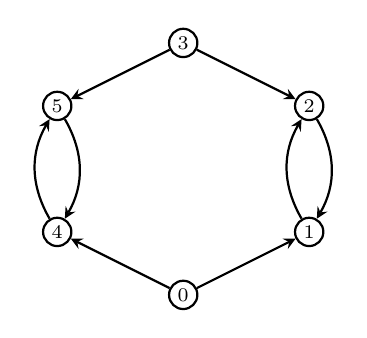
\begin{tikzpicture}
[arrowDecorate/.style={->,>=stealth,thick},%
  nodeDecorate/.style={shape=circle,inner sep=1.5pt,draw,thick},%
  scale=0.8]
\scriptsize
%% nodes or vertices
\foreach \nodename/\x/\y in {1/2/1, 2/2/3, 3/0/4, 0/0/0, 4/-2/1, 5/-2/3}
{
  \node (\nodename) at (\x,\y) [nodeDecorate] {$\nodename$};
}
%% edges or lines
\path
(1) edge[arrowDecorate,bend left] node {} (2)
(2) edge[arrowDecorate,bend left] node {} (1)
(3) edge[arrowDecorate] node {} (2)
(3) edge[arrowDecorate] node {} (5)
(0) edge[arrowDecorate] node {} (1)
(0) edge[arrowDecorate] node {} (4)
(4) edge[arrowDecorate,bend left] node {} (5)
(5) edge[arrowDecorate,bend left] node {} (4);
\end{tikzpicture}
%%
%%
\qquad\qquad
%%
%%
\begin{tikzpicture}
\node at (0,0) {%
$
\begin{bmatrix}
0      & 1      & 2      & \infty & 1      & 2 \\
\infty & 0      & 1      & \infty & \infty & \infty \\
\infty & 1      & 0      & \infty & \infty & \infty \\
\infty & 2      & 1      & 0      & 2      & 1 \\
\infty & \infty & \infty & \infty & 0      & 1 \\
\infty & \infty & \infty & \infty & 1      & 0
\end{bmatrix}
$
};
\end{tikzpicture}
}
%%
%%
\qquad
%% graph
\subfigure[]{
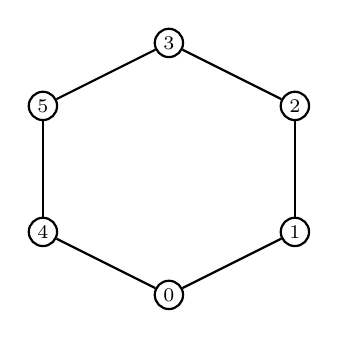
\begin{tikzpicture}
[lineDecorate/.style={-,thick},%
  nodeDecorate/.style={shape=circle,inner sep=1.5pt,draw,thick},%
  scale=0.8]
\scriptsize
%% nodes or vertices
\foreach \nodename/\x/\y in {1/2/1, 2/2/3, 3/0/4, 0/0/0, 4/-2/1, 5/-2/3}
{
  \node (\nodename) at (\x,\y) [nodeDecorate] {$\nodename$};
}
%% edges or lines
\path
\foreach \startnode/\endnode in {1/2, 1/0, 2/3, 3/5, 0/4, 4/5}
{
  (\startnode) edge[lineDecorate] node {} (\endnode)
};
\end{tikzpicture}
%%
%%
\qquad\qquad
%%
%%
\begin{tikzpicture}
\node at (0,0) {%
$
\begin{bmatrix}
0 & 1 & 2 & 3 & 1 & 2 \\
1 & 0 & 1 & 2 & 2 & 3 \\
2 & 1 & 0 & 1 & 3 & 2 \\
3 & 2 & 1 & 0 & 2 & 1 \\
1 & 2 & 3 & 2 & 0 & 1 \\
2 & 3 & 2 & 1 & 1 & 0
\end{bmatrix}
$
};
\end{tikzpicture}
}

\caption{Distance matrices of directed and undirected graphs.}
\label{fig:distance_connectivity:distance_matrix_directed_undirected_graphs}
\end{figure}

Instead of one distance matrix, we can define several distance
matrices on $G$. Consider an edge-weighted graph $G = (V,E)$ without
negative weight cycles and let
\[
d: V \times V \to \R \cup \{\infty\}
\]
be a distance function of $G$. Let $\partial = \diam(G)$ be the
diameter of $G$ and index the vertices of $G$ in some arbitrary but
fixed manner, say $V = \{v_0, v_1, \dots, v_n\}$. The sequence of
\emph{distance matrices}\index{matrix!distance} of $G$ are a sequence
of $(n - 1) \times (n - 1)$ matrices $A_1, A_2, \dots, A_\partial$ where
\[
(A_k)_{ij}
=
\begin{cases}
1, & \text{if $d(v_i, v_j) = k$}, \\[4pt]
0, & \text{otherwise}.
\end{cases}
\]
In particular, $A_1$ is the usual adjacency matrix $A$. To compute the
sequence of distance matrices of $G$, use the
Floyd-Roy-Warshall\index{Floyd-Roy-Warshall algorithm} algorithm to
compute the distance between each pair of vertices and assign the
resulting distance to the corresponding matrix $A_i$.

The distance matrix arises in several applications, including
communication network design~\cite{GrahamPollak1971} and network flow
algorithms~\cite{Dijkstra1959}. Thanks to
Graham\index{Graham, Ronald L.} and
Pollak\index{Pollak, O.}~\cite{GrahamPollak1971}, the following
unusual fact is known. If $T$ is any tree then
\[
\det D(T)
=
(-1)^{n - 1} (n - 1) 2^{n - 2}
\]
where $n$ denotes the order of $T$. In particular, the determinant of
the distance matrix of a tree is independent of the structure of the
tree.  This fact is proven in the paper~\cite{GrahamPollak1971}, but
see also~\cite{EdelbergEtAl1976}.


%%%%%%%%%%%%%%%%%%%%%%%%%%%%%%%%%%%%%%%%%%%%%%%%%%%%%%%%%%%%%%%%%%%%%%%%%%%

\section{Vertex and edge connectivity}

If $G = (V,E)$ is a graph and $U \subseteq V$ is a vertex set with the
property that $G - U$ has more connected components than $G$, then we
call $U$ a \emph{vertex-cut}\index{vertex-cut}. The term
\emph{cut-vertex}\index{cut-vertex} or
\emph{cut-point}\index{cut-point} is used when the vertex-cut consists
of exactly one vertex. For an intuitive appreciation of vertex-cut,
suppose $G = (V,E)$ is a connected graph. Then $U \subseteq V$ is a
vertex-cut if the vertex\index{vertex!deletion subgraph} deletion
subgraph $G - U$ is disconnected. For example, the cut-vertex of the
graph in Figure~\ref{fig:distance_connectivity:claw_graph} is the
vertex $0$. By $\kappa_v(G)$\index{$\kappa_v(G)$} we mean the
\emph{vertex connectivity}\index{vertex connectivity} of a connected
graph $G$, defined as the minimum number of vertices whose removal
would either disconnect $G$ or reduce $G$ to the trivial graph. The
vertex connectivity $\kappa_v(G)$ is also written as
$\kappa(G)$\index{$\kappa(G)$}. The vertex connectivity of the graph
in Figure~\ref{fig:distance_connectivity:claw_graph} is
$\kappa_v(G) = 1$ because we only need to remove vertex $0$ in order
to disconnect the graph. The vertex connectivity of a connected graph
$G$ is thus the vertex-cut of minimum cardinality. And $G$ is said to
be $k$-\emph{connected}\index{$k$-connected} if $\kappa_v(G) \geq k$.
From the latter definition, it immediately follows that if $G$ has at
least $3$ vertices and is $k$-connected then any vertex-cut of $G$ has
at least cardinality $k$. For instance, the graph in
Figure~\ref{fig:distance_connectivity:claw_graph} is $1$-connected. In
other words, $G$ is $k$-connected if the graph remains connected even
after removing any $k - 1$ or fewer vertices from $G$.

\begin{figure}[!htbp]
\centering
\index{cut-edge}
\index{cut-vertex}
\index{claw graph}
%%%%%%%%%%%%%%%%%%%%%%%%%%%%%%%%%%%%%%%%%%%%%%%%%%%%%%%%%%%%%%%%%%%%%%%%%%%
%% This file is part of the book
%%
%% Algorithmic Graph Theory
%% http://code.google.com/p/graph-theory-algorithms-book/
%%
%% Copyright (C) 2009, 2010, 2011 Minh Van Nguyen <nguyenminh2@gmail.com>
%%
%% See the file COPYING for copying conditions.
%%%%%%%%%%%%%%%%%%%%%%%%%%%%%%%%%%%%%%%%%%%%%%%%%%%%%%%%%%%%%%%%%%%%%%%%%%%

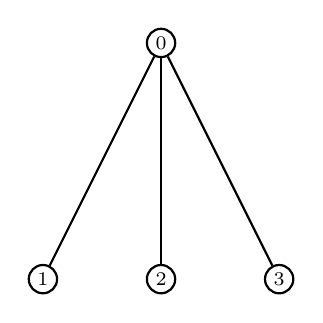
\begin{tikzpicture}
[nodeDecorate/.style={shape=circle,inner sep=1.5pt,draw,thick},%
  lineDecorate/.style={-,thick},%
  scale=1.5]
\scriptsize
%% nodes or vertices
\foreach \nodename/\x/\y in {1/0/0, 2/1/0, 3/2/0, 0/1/2}
{
  \node (\nodename) at (\x,\y) [nodeDecorate] {$\nodename$};
}
%% edges or lines
\path
\foreach \startnode/\endnode in {0/1, 0/2, 0/3} {
  (\startnode) edge[lineDecorate] node {} (\endnode)
};
\end{tikzpicture}

\caption{A claw graph with $4$ vertices.}
\label{fig:distance_connectivity:claw_graph}
\end{figure}

\begin{figure}[!htbp]
\centering
\index{Petersen!graph}
%%%%%%%%%%%%%%%%%%%%%%%%%%%%%%%%%%%%%%%%%%%%%%%%%%%%%%%%%%%%%%%%%%%%%%%%%%%
%% This file is part of the book
%%
%% Algorithmic Graph Theory
%% http://code.google.com/p/graph-theory-algorithms-book/
%%
%% Copyright (C) 2009, 2010, 2011 Minh Van Nguyen <nguyenminh2@gmail.com>
%%
%% See the file COPYING for copying conditions.
%%%%%%%%%%%%%%%%%%%%%%%%%%%%%%%%%%%%%%%%%%%%%%%%%%%%%%%%%%%%%%%%%%%%%%%%%%%

\documentclass{article}

\usepackage{tikz}
\usetikzlibrary{external}
\tikzexternalize{petersen-graph}

\begin{document}

\begin{figure}
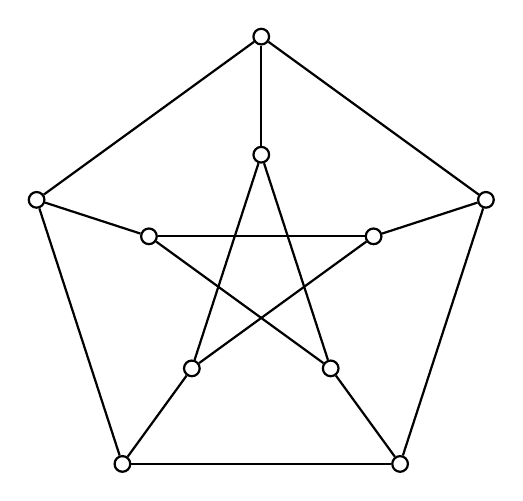
\begin{tikzpicture}
[nodeDecorate/.style={shape=circle,inner sep=2pt,draw,thick},%
  lineDecorate/.style={-,thick},scale=1.5]
%% nodes or vertices
\foreach \nodename/\x/\y in {
  %% outer pentagon
  0/0/2, 1/-1.9021/0.6180, 2/-1.1755/-1.6180, 3/1.1755/-1.6180,
  4/1.9021/0.6180,
  %% inner pentagon
  5/0/1, 6/-0.9510/0.3090, 7/-0.5877/-0.8090, 8/0.5877/-0.8090,
  9/0.9510/0.3090}
{
  \node (\nodename) at (\x,\y) [nodeDecorate] {};
}
%% edges or lines
\path
\foreach \startnode/\endnode in {0/1, 0/4, 0/5, 1/2, 1/6, 2/3, 2/7,
  3/4, 3/8, 4/9, 5/7, 5/8, 6/8, 6/9, 7/9}
{
  (\startnode) edge[lineDecorate] node {} (\endnode)
};
\end{tikzpicture}
\end{figure}

\end{document}

\caption{The Petersen graph on $10$ vertices.}
\label{fig:distance_connectivity:petersen_graph}
\end{figure}

\begin{example}
\rm
Here is a Sage example concerning $\kappa(G)$ using the
Petersen\index{Petersen!graph} graph depicted in
Figure~\ref{fig:distance_connectivity:petersen_graph}. A linear
programming Sage package, such as GLPK, must be installed for the
commands below to work.
%%
\begin{lstlisting}
sage: G = graphs.PetersenGraph()
sage: len(G.vertices())
10
sage: G.vertex_connectivity()
3.0
sage: G.delete_vertex(0)
sage: len(G.vertices())
9
sage: G.vertex_connectivity()
2.0
\end{lstlisting}
\qed
\end{example}

The notions of edge-cut and cut-edge are similarly defined. Let
$G = (V,E)$ be a graph and $D \subseteq E$ an edge set such that the
edge deletion subgraph $G - D$ has more components than $G$. Then $D$
is called an \emph{edge-cut}\index{edge-cut}. An edge-cut $D$ is said
to be \emph{minimal} if no proper subset of $D$ is an edge-cut. The
term \emph{cut-edge}\index{cut-edge} or \emph{bridge}\index{bridge} is
reserved for the case where the set $D$ is a singleton. Think of a
cut-edge as an edge whose removal from a connected graph would result
in that graph being disconnected. Going back to the case of the graph
in Figure~\ref{fig:distance_connectivity:claw_graph}, each edge of the
graph is a cut-edge. A graph having no cut-edge is called
\emph{bridgeless}\index{bridgeless}. An open question as of~2010
involving bridges is the
\emph{cycle double cover conjecture}\index{cycle double cover conjecture},
due to Paul Seymour\index{Seymour!Paul} and G.~Szekeres\index{Szekeres, G.},
which states that every bridgeless graph admits a set of cycles that
contains each edge exactly twice. The \emph{edge connectivity} of a
connected graph $G$, written $\kappa_e(G)$\index{$\kappa_e(G)$} and
sometimes denoted by $\lambda(G)$\index{$\lambda(G)$}, is the minimum
number of edges whose removal would disconnect $G$. In other words,
$\kappa_e(G)$ is the minimum cardinality among all edge-cuts of
$G$. Furthermore, $G$ is said to be
$k$-\emph{edge-connected}\index{$k$-edge-connected} if
$\kappa_e(G) \geq k$. A connected graph that is $k$-edge-connected is
guaranteed to be connected after removing $\leq k - 1$ edges from
it. When we have removed $k$ or more edges, then the graph would
become disconnected. By convention, a $1$-edge-connected graph is
simply a connected graph. The graph in
Figure~\ref{fig:distance_connectivity:claw_graph} has edge
connectivity $\kappa_e(G) = 1$ and is $1$-edge-connected.

\begin{example}
\rm
Here is a Sage example concerning $\lambda(G)$ using the
Petersen\index{Petersen!graph} graph shown in
Figure~\ref{fig:distance_connectivity:petersen_graph}. You must
install an optional linear programming Sage package such as GLPK for
the commands below to work.
%%
\begin{lstlisting}
sage: G = graphs.PetersenGraph()
sage: len(G.vertices())
10
sage: E = G.edges(); len(E)
15
sage: G.edge_connectivity()
3.0
sage: G.delete_edge(E[0])
sage: len(G.edges())
14
sage: G.edge_connectivity()
2.0
\end{lstlisting}
\qed
\end{example}

Vertex and edge connectivity are intimately related to the reliability
and survivability of computer networks. If a computer network
$G$~(which is a connected graph) is $k$-connected, then it would
remain connected despite the failure of at most $k - 1$ network
nodes. Similarly, $G$ is $k$-edge-connected if the network remains
connected after the failure of at most $k - 1$ network links. In
practical terms, a network with redundant nodes and/or links can
afford to endure the failure of a number of nodes and/or links and
still be connected, whereas a network with very few redundant nodes
and/or links~(e.g. something close to a spanning tree) is more prone
to be disconnected. A $k$-connected or $k$-edge-connected network is
more robust (i.e. can withstand) against node and/or link failures
than is a $j$-connected or $j$-edge-connected network, where $j < k$.

\begin{proposition}
\label{prop:distance_connectivity:edge_degree_inequality}
If $\delta(G)$ is the minimum degree of an undirected connected graph
$G = (V,E)$, then the edge connectivity of $G$ satisfies
$\lambda(G) \leq \delta(G)$.
\end{proposition}

\begin{proof}
Choose a vertex $v \in V$ whose degree is
$\deg(v) = \delta(G)$. Deleting the $\delta(G)$ edges incident on $v$
suffices to disconnect $G$ as $v$ is now an isolated vertex. It is
possible that $G$ has an edge-cut whose cardinality is smaller than
$\delta(G)$. Hence the result follows.
\end{proof}

Let $G = (V,E)$ be a graph and suppose $X_1$ and $X_2$ comprise a
partition of $V$. A \emph{partition-cut} of $G$, denoted
$\langle X_1, X_2 \rangle$, is the set of all edges of $G$ with one
endpoint in $X_1$ and the other endpoint in $X_2$. If $G$ is a
bipartite graph with bipartition $X_1$ and $X_2$, then
$\langle X_1, X_2 \rangle$ is a partition-cut of $G$. It follows that
a partition-cut is also an edge-cut.

\begin{proposition}
An undirected connected graph $G$ is $k$-edge-connected if and only if
any partition-cut of $G$ has at least $k$ edges.
\end{proposition}

\begin{proof}
Assume that $G$ is $k$-edge-connected. Then each edge-cut has at least
$k$ edges. As a partition-cut is an edge-cut, then any partition-cut
of $G$ has at least $k$ edges.

On the other hand, suppose each partition-cut has at least $k$
edges. If $D$ is a minimal edge-cut of $G$ and $X_1$ and $X_2$ are the
vertex sets of the two components of $G - D$, then
$D = \langle X_1, X_2 \rangle$. To see this, note that
$D \subseteq \langle X_1, X_2 \rangle$. If
$\langle X_1, X_2 \rangle - D \neq \emptyset$ then choose some
$e \in \langle X_1, X_2 \rangle$ such that $e \notin D$. The endpoints
of $e$ belong to the same component of $G - D$, in contradiction of
the definition of $X_1$ and $X_2$. Thus any minimal edge-cut is a
partition-cut and conclude that any edge-cut has at least $k$ edges.
\end{proof}

%% NOTE: need to polish up statement and proof of Bondy's theorem.
%% \begin{theorem}
%% (Bondy's theorem)
%% {\rm
%% Suppose

%% \begin{itemize}
%% \item
%% $G=(V,E)$ is a connected simple graph with $n=|V|$,
%% \item
%% $0<k<n$,
%% \item
%% the (non-decreasing) degree sequence
%% $[d_1,d_2,\dots, d_n]$ satisfies
%% $d_j\geq j+k-1$, for $1\leq j\leq n-1-d_{n-k+1}$,
%% \end{itemize}
%% then $G$ is $k$-vertex-connected.
%% }
%% \end{theorem}
%% \index{Bondy's theorem}

%% \begin{proof}[Solution]
%% Suppose not, so $\kappa(G)<k$. Then there exists an
%% $S\subset V$, $|S|=s<k$, such that $G'=G-S$ has more
%% than one connected component. Let $H$ be connected
%% component of $G'$ of minimal number of
%% vertices, $j=V(H)$. If $v\in V(H)$ then
%% $\deg_G(v)\leq j-1+s$, since $v$ is not adjacent to any
%% vertex in any other connected component of $G'$.

%% Since $H$ was chosen minimally, $j\leq n-s-j$, so
%% $\deg_G(v)\leq n-j-1$. This proves the following claim.

%% \noindent
%% {\bf Claim}: If $\deg_G(v) > n-j-1$ then $v\in S$.

%% A vertex of degree $d_{n-s}$ cannot belong to
%% $S$ because $S$ has $|S|=s$ vertices and the
%% vertices of degree $d_n$, $d_{n-1}$, \dots,
%% $d_{n-s-1}$ already exhaust the vertices in $S$. Therefore,

%% \[
%% d_{n-s}\leq n-j-1.
%% \]
%% We have $s\leq k-1$, so $d_{n-(k-1)}\leq d_{n-s}\leq n-j-1$,
%% so $j\leq n-1-d_{n-k+1}$.

%% Recall $v\in V(H)$ implies $\deg_G(v)\leq j-1+s$.
%% Since $j=|V(H)|$, we have
%% $d_j\leq j-1-s$.
%% By hypothesis, $d_j\geq j+k-1$, so together we have

%% \[
%% j+k-1\leq d_j \leq j-1+s.
%% \]
%% This forces $k\leq s$, a contradiction.
%% \end{proof}

\begin{proposition}
\label{prop:distance_connectivity:vertex_edge_inequality}
If $G = (V,E)$ is an undirected connected graph with vertex
connectivity $\kappa(G)$ and edge connectivity $\lambda(G)$, then we
have $\kappa(G) \leq \lambda(G)$.
\end{proposition}

\begin{proof}
Let $S$ be an edge-cut of $G$ with cardinality
$k = |S| = \lambda(G)$. Removing $k$ suitably chosen vertices of $G$
suffice to delete the edges of $S$ and hence disconnect $G$. It is
also possible to have a smaller vertex-cut elsewhere in $G$. Hence the
inequality follows.
\end{proof}

Taking together
Propositions~\ref{prop:distance_connectivity:edge_degree_inequality}
and~\ref{prop:distance_connectivity:vertex_edge_inequality}, we have
Whitney's\index{Whitney!inequality} inequality.

\begin{theorem}
\textbf{Whitney's inequality~\cite{Whitney1932}.}\index{Whitney!inequality}
Let $G$ be an undirected connected graph with vertex connectivity
$\kappa(G)$, edge connectivity $\lambda(G)$, and minimum degree
$\delta(G)$. Then we have the following inequality:
\[
\kappa(G)
\leq
\lambda(G)
\leq
\delta(G).
\]
\end{theorem}

\begin{proposition}
\label{prop:distance_connectivity:edge_removal_subgraph_k_minus_1_connected}
Let $G$ be an undirected connected graph that is $k$-connected for
some $k \geq 3$. If $e$ is an edge of $G$, then the edge-deletion
subgraph $G - e$ is $(k - 1)$-connected.
\end{proposition}

\begin{proof}
Let $V = \{v_1, v_2, \dots, v_{k-2}\}$ be a set of $k - 2$ vertices in
$G - e$. It suffice to show the existence of a $u$-$v$ walk in
$(G - e) - V$ for any distinct vertices $u$ and $v$ in
$(G - e) - V$. We need to consider two cases:~(i) at least one of the
endpoints of $e$ is in $V$; and~(ii) neither endpoints of $e$ is in
$V$.

(i)~Assume that $V$ has at least one endpoint of $e$. As $G - V$ is
$2$-connected, any distinct pair of vertices $u$ and $v$ in $G - V$ is
connected by a $u$-$v$ path that excludes $e$. Hence the $u$-$v$ path
is also in $(G - e) - V$.

(ii)~Assume that neither endpoints of $e$ is in $V$. If $u$ and $v$
are distinct vertices in $(G - e) - V$, then either:~(1) both $u$ and
$v$ are endpoints of $e$; or~(2) at least one of $u$ and $v$ is an
endpoint of $e$.
%%
\begin{enumerate}[(1)]
\item Suppose $u$ and $v$ are both endpoints of $e$. As $G$ is
  $k$-connected, then $G$ has at least $k + 1$ vertices so that the
  vertex set of $G - \{v_1, v_2, \dots, v_{k-2}, u, v\}$ is
  nonempty. Let $w$ be a vertex of
  $G - \{v_1, v_2, \dots, v_{k-2}, u, v\}$. Then there is a $u$-$w$
  path in $G - \{v_1, v_2, \dots, v_{k-2}, v\}$ and a $w$-$v$ path in
  $G - \{v_1, v_2, \dots, v_{k-2}, u\}$. Neither the $u$-$w$ nor the
  $w$-$v$ paths contain $e$. The concatenation of these two paths is a
  $u$-$v$ walk in $(G - e) - V$.

\item Now suppose at least one of $u$ and $v$, say $u$, is an endpoint
  of $e$. Let $w$ be the other endpoint of $e$. As $G$ is
  $k$-connected, then $G - \{v_1, v_2, \dots, v_{k-2}, w\}$ is
  connected and we can find a $u$-$v$ path $P$ in
  $G - \{v_1, v_2, \dots, v_{k-2}, w\}$. Furthermore $P$ is a $u$-$v$
  path in $G - \{v_1, v_2, \dots, v_{k-2}\}$ that neither contain $w$
  nor $e$. Hence $P$ is a $u$-$v$ path in $(G - e) - V$.
\end{enumerate}
%%
Conclude that $G - e$ is $(k - 1)$-connected.
\end{proof}

Repeated application of
Proposition~\ref{prop:distance_connectivity:edge_removal_subgraph_k_minus_1_connected}
results in the following corollary.

\begin{corollary}
Let $G$ be an undirected connected graph that is $k$-connected for
some $k \geq 3$. If $E$ is any set of $m$ edges of $G$, for
$m \leq k - 1$, then the edge-deletion subgraph $G - E$ is
$(k - m)$-connected.
\end{corollary}

What does it mean for a communications\index{communications network}
network to be fault-tolerant\index{fault-tolerant}? In~1932,
Hassler\index{Whitney!Hassler} Whitney provided~\cite{Whitney1932} a
characterization of $2$-connected graphs whereby he showed that a
graph $G$ is $2$-connected if and only if each pair of distinct
vertices in $G$ has two different paths connecting those two
vertices. A key to understanding Whitney's characterization of
$2$-connected graphs is the notion of internal vertex of a path. Given
a path $P$ in a graph, a vertex along that path is said to be an
\emph{internal vertex}\index{vertex!internal} if it is neither the
initial nor the final vertex of $P$. In other words, a path $P$ has an
internal vertex if and only if $P$ has at least two edges. Building
upon the notion of internal vertices, we now discuss what it means for
two paths to be internally disjoint. Let $u$ and $v$ be distinct
vertices in a graph $G$ and suppose $P_1$ and $P_2$ are two paths from
$u$ to $v$. Then $P_1$ and $P_2$ are said to be
\emph{internally disjoint}\index{path!internally disjoint} if they
do not share any common internal vertex. Two $u$-$v$ paths are
internally disjoint in the sense that both $u$ and $v$ are the only
vertices to be found in common between those paths. The notion of
internally disjoint paths can be easily extended to a collection of
$u$-$v$ paths. Whitney's characterization essentially says that a
graph is $2$-connected if and only if any two $u$-$v$ paths are
internally disjoint.

Consider the notion of internally disjoint paths within the context of
communications\index{communications network} network. As a first
requirement for fault-tolerant communications network, we want the
network to remain connected despite the failure of any network
node. By Whitney's characterization, this is possible if the original
communications network is $2$-connected. That is, we say that a
communications network is \emph{fault-tolerant}\index{fault-tolerant}
provided that any pair of distinct nodes is connected by two
internally disjoint paths. The failure of any node should at least
guarantee that any two distinct nodes are still connected.

\begin{theorem}
\label{thm:distance_connectivity:Whitney_characterization_2_connected_graphs}
\textbf{Whitney's characterization of $2$-connected graphs~\cite{Whitney1932}.}
Let $G$ be an undirected connected graph having at least $3$
vertices. Then $G$ is $2$-connected if and only if any two distinct
vertices in $G$ are connected by two internally disjoint paths.
\end{theorem}

\begin{proof}
($\Longleftarrow$)
For the case of necessity, argue by contraposition. That is, suppose
$G$ is not $2$-connected. Let $v$ be a cut-vertex of $G$, from which
it follows that $G - v$ is disconnected. We can find two vertices $w$
and $x$ such that there is no $w$-$x$ path in $G - v$. Therefore $v$
is an internal vertex of any $w$-$x$ path in $G$.

($\Longrightarrow$)
For the case of sufficiency, let $G$ be $2$-connected and let $u$ and
$v$ be any two distinct vertices in $G$. Argue by induction on
$d(u,v)$ that $G$ has at least two internally disjoint $u$-$v$
paths. For the base case, suppose $u$ and $v$ are connected by an edge
$e$ so that $d(u,v) = 1$. Adapt the proof of
Proposition~\ref{prop:distance_connectivity:edge_removal_subgraph_k_minus_1_connected}
to see that $G - e$ is connected. Hence we can find a $u$-$v$ path $P$
in $G - e$ such that $P$ and $e$ are two internally disjoint $u$-$v$
paths in $G$.

Assume for induction that $G$ has two internally disjoint $u$-$v$
paths where $d(u,v) < k$ for some $k \geq 2$. Let $w$ and $x$ be two
distinct vertices in $G$ such that $d(w,x) = k$ and hence there is a
$w$-$x$ path in $G$ of length $k$, i.e. we have a $w$-$x$ path
\[
W: w = w_1, w_2, \dots, w_{k-1}, w_k = x.
\]
Note that $d(w, w_{k-1}) < k$ and apply the induction hypothesis to
see that we have two internally disjoint $w$-$w_{k-1}$ paths in $G$;
call these paths $P$ and $Q$. As $G$ is $2$-connected, we have a
$w$-$x$ path $R$ in $G - w_{k-1}$ and hence $R$ is also a $w$-$x$ path
in $G$. Let $z$ be the vertex on $R$ that immediately precedes $x$ and
assume without loss of generality that $z$ is on $P$. We claim that
$G$ has two internally disjoint $w$-$x$ paths. One of these paths is
the concatenation of the subpath of $P$ from $w$ to $z$ with the
subpath of $R$ from $z$ to $x$. If $x$ is not on $Q$, then construct a
second $w$-$x$ path, internally disjoint from the first one, as
follows: concatenate the path $Q$ with the edge $w_{k-1} w$. In case
$x$ is on $Q$, take the subpath of $Q$ from $w$ to $x$ as the required
second path.
\end{proof}

From
Theorem~\ref{thm:distance_connectivity:Whitney_characterization_2_connected_graphs},
an undirected connected graph $G$ is $2$-connected if and only if any
two distinct vertices of $G$ are connected by two internally disjoint
paths. In particular, let $u$ and $v$ be any two distinct vertices of
$G$ and let $P$ and $Q$ be two internally disjoint $u$-$v$ paths as
guaranteed by
Theorem~\ref{thm:distance_connectivity:Whitney_characterization_2_connected_graphs}.
Starting from $u$, travel along the path $P$ to arrive at $v$. Then
start from $v$ and travel along the path $Q$ to arrive at $u$. The
concatenation of the internally disjoint paths $P$ and $Q$ is hence a
cycle passing through $u$ and $v$. We have proved the following
corollary to
Theorem~\ref{thm:distance_connectivity:Whitney_characterization_2_connected_graphs}.

\begin{corollary}
Let $G$ be an undirected connected graph having at least $3$
vertices. Then $G$ is $2$-connected if and only if any two distinct
vertices of $G$ lie on a common cycle.
\end{corollary}

The following theorem provides further characterizations of
$2$-connected graphs, in addition to Whitney's characterization.

\begin{theorem}
\label{thm:distance_connectivity:characterization_2_connected_graphs}
\textbf{Characterizations of $2$-connected graphs.}
Let $G = (V,E)$ be an undirected connected graph having at least $3$
vertices. Then the following are equivalent.
%%
\begin{enumerate}
\item $G$ is $2$-connected.

\item If $u,v \in V$ are distinct vertices of $G$, then $u$ and $v$
  lie on a common cycle.

\item If $v \in V$ and $e \in E$, then $v$ and $e$ lie on a common
  cycle.

\item If $e_1, e_2 \in E$ are distinct edges of $G$, then $e_1$ and
  $e_2$ lie on a common cycle.

\item If $u,v \in V$ are distinct vertices and $e \in E$, then they
  lie on a common path.

\item If $u,v,w \in V$ are distinct vertices, then they lie on a
  common path.

\item If $u,v,w \in V$ are distinct vertices, then there is a path
  containing any two of these vertices but excluding the third.
\end{enumerate}
\end{theorem}


%%%%%%%%%%%%%%%%%%%%%%%%%%%%%%%%%%%%%%%%%%%%%%%%%%%%%%%%%%%%%%%%%%%%%%%%%%%

\section{Menger's theorem}
\index{Menger's theorem}

Menger's theorem has a number of different versions: an undirected,
vertex-connectivity version; a directed, vertex-connectivity version;
an undirected, edge-connectivity version; and a directed,
edge-connectivity version. In this section, we will prove the
undirected, vertex-connectivity version. But first, let's consider a
few technical results that will be of use for the purpose of this
section.

Let $u$ and $v$ be distinct vertices in a connected graph $G = (V,E)$
and let $S \subseteq V$. Then $S$ is said to be $u$-$v$
\emph{separating} if $u$ and $v$ lie in different components of the
vertex deletion subgraph $G - S$. The vertices $u$ and $v$ are
positioned such that after removing vertices in $S$ from $G$ and the
corresponding edges, $u$ and $v$ are no longer connected nor strongly
connected to each other. It is clear by definition that
$u,v \notin S$. We also say that $S$ \emph{separates} $u$ and
$v$, or $S$ is a vertex separating set. Similarly an edge set
$T \subseteq E$ is $u$-$v$ separating~(or separates $u$ and $v$) if
$u$ and $v$ lie in different components of the edge deletion subgraph
$G - T$. But unlike the case of vertex separating sets, it is possible
for $u$ and $v$ to be endpoints of edges in $T$ because the removal of
edges does not result in deleting the corresponding endpoints. The set
$T$ is also called an edge separating set. In other words, $S$ is a
vertex cut\index{vertex!cut} and $T$ is an edge
cut\index{edge!cut}. When it is clear from context, we simply refer to
a separating\index{separating set} set. See
Figure~\ref{fig:distance_connectivity:vertex_edge_separating_sets} for
illustrations of separating sets.

\begin{figure}[!htbp]
\centering
\index{separating set}
%%%%%%%%%%%%%%%%%%%%%%%%%%%%%%%%%%%%%%%%%%%%%%%%%%%%%%%%%%%%%%%%%%%%%%%%%%%
%% This file is part of the book
%%
%% Algorithmic Graph Theory
%% http://code.google.com/p/graph-theory-algorithms-book/
%%
%% Copyright (C) 2009, 2010, 2011 Minh Van Nguyen <nguyenminh2@gmail.com>
%%
%% See the file COPYING for copying conditions.
%%%%%%%%%%%%%%%%%%%%%%%%%%%%%%%%%%%%%%%%%%%%%%%%%%%%%%%%%%%%%%%%%%%%%%%%%%%

\subfigure[Original graph.]{
\label{fig:separating_set:original_graph}
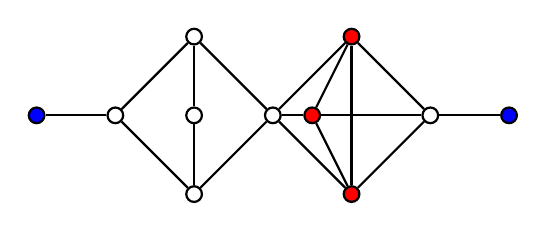
\begin{tikzpicture}
[nodeDecorate/.style={shape=circle,inner sep=2pt,draw,thick},%
  lineDecorate/.style={-,thick},scale=1]
%% nodes or vertices
\foreach \nodename/\x/\y in {
  0/0/0, 2/2/0, 6/-1/1, 7/-1/0, 8/-1/-1, 9/-2/0}
{
  \node (\nodename) at (\x,\y) [nodeDecorate] {};
}
\foreach \nodename/\x/\y/\fillcolor in {
  1/0.5/0/red, 3/3/0/blue, 4/1/-1/red, 5/1/1/red, 10/-3/0/blue}
{
  \node (\nodename) at (\x,\y) [nodeDecorate,fill=\fillcolor] {};
}
%% edges or lines
\path
\foreach \startnode/\endnode in {
  0/1, 0/4, 0/5, 0/6, 0/8, 1/2, 1/4, 1/5, 2/3, 2/4, 2/5, 4/5, 6/7,
  6/9, 7/8, 8/9, 9/10}
{
  (\startnode) edge[lineDecorate] node {} (\endnode)
};
\end{tikzpicture}
}
%%
%%
\qquad
\subfigure[Vertex separated.]{
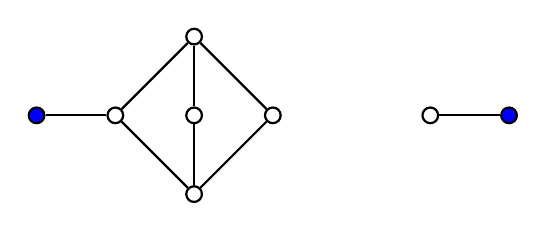
\begin{tikzpicture}
[nodeDecorate/.style={shape=circle,inner sep=2pt,draw,thick},%
  lineDecorate/.style={-,thick},scale=1]
%% nodes or vertices
\foreach \nodename/\x/\y in {
  0/0/0, 2/2/0, 6/-1/1, 7/-1/0, 8/-1/-1, 9/-2/0}
{
  \node (\nodename) at (\x,\y) [nodeDecorate] {};
}
\node (3) at (3,0) [nodeDecorate,fill=blue] {};
\node (10) at (-3,0) [nodeDecorate,fill=blue] {};
%% edges or lines
\path
\foreach \startnode/\endnode in {
  0/6, 0/8, 2/3, 6/7, 6/9, 7/8, 8/9, 9/10}
{
  (\startnode) edge[lineDecorate] node {} (\endnode)
};
\end{tikzpicture}
}
%%
%%
\subfigure[Original graph.]{
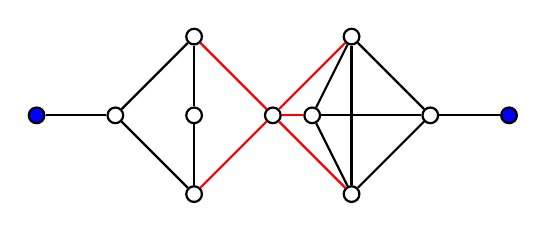
\begin{tikzpicture}
[nodeDecorate/.style={shape=circle,inner sep=2pt,draw,thick},%
  lineDecorate/.style={-,thick},scale=1]
%% nodes or vertices
\foreach \nodename/\x/\y in {
  0/0/0, 1/0.5/0, 2/2/0, 4/1/-1, 5/1/1, 6/-1/1, 7/-1/0, 8/-1/-1, 9/-2/0}
{
  \node (\nodename) at (\x,\y) [nodeDecorate] {};
}
\node (3) at (3,0) [nodeDecorate,fill=blue] {};
\node (10) at (-3,0) [nodeDecorate,fill=blue] {};
%% edges or lines
\path
\foreach \startnode/\endnode in {
  1/2, 1/4, 1/5, 2/3, 2/4, 2/5, 4/5, 6/7, 6/9, 7/8, 8/9, 9/10}
{
  (\startnode) edge[lineDecorate] node {} (\endnode)
}
\foreach \startnode/\endnode/\edgecolor in { 0/1, 0/4, 0/5, 0/6, 0/8}
{
  (\startnode) edge[lineDecorate,color=red] node {} (\endnode)
};
\end{tikzpicture}
}
%%
%%
\qquad
\subfigure[Edge separated.]{
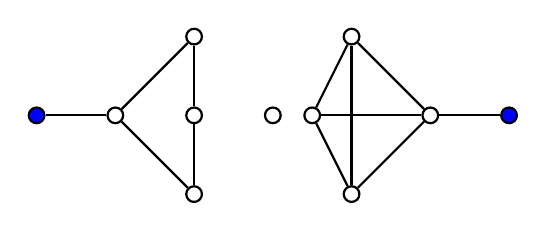
\begin{tikzpicture}
[nodeDecorate/.style={shape=circle,inner sep=2pt,draw,thick},%
  lineDecorate/.style={-,thick},scale=1]
%% nodes or vertices
\foreach \nodename/\x/\y in {
  0/0/0, 1/0.5/0, 2/2/0, 4/1/-1, 5/1/1, 6/-1/1, 7/-1/0, 8/-1/-1, 9/-2/0}
{
  \node (\nodename) at (\x,\y) [nodeDecorate] {};
}
\node (3) at (3,0) [nodeDecorate,fill=blue] {};
\node (10) at (-3,0) [nodeDecorate,fill=blue] {};
%% edges or lines
\path
\foreach \startnode/\endnode in {
  1/2, 1/4, 1/5, 2/3, 2/4, 2/5, 4/5, 6/7, 6/9, 7/8, 8/9, 9/10}
{
  (\startnode) edge[lineDecorate] node {} (\endnode)
};
\end{tikzpicture}
}

\caption{Vertex and edge separating sets. Blue-colored vertices are
  those we want to separate. The red-colored vertices form a vertex
  separating set or vertex cut\index{vertex!cut}; the red-colored
  edges constitute an edge separating set or edge cut\index{edge!cut}.}
\label{fig:distance_connectivity:vertex_edge_separating_sets}
\end{figure}

\begin{proposition}
\label{prop:distance_connectivity:upper_bound_internally_disjoint_paths}
Consider two distinct, non-adjacent vertices $u,v$ in a connected
graph $G$. If $\cP_{uv}$ is a collection of internally disjoint
$u$-$v$ paths in $G$ and $S_{uv}$ is a $u$-$v$ separating set of
vertices in $G$, then
%%
\begin{equation}
\label{eqn:distance_connectivity:upper_bound_internally_disjoint_paths}
|\cP_{uv}| \leq |S_{uv}|.
\end{equation}
\end{proposition}

\begin{proof}
Each $u$-$v$ path in $\cP_{uv}$ must include at least one vertex from
$S_{uv}$ because $S_{uv}$ is a vertex cut of $G$. Any two distinct
paths in $\cP_{uv}$ cannot contain the same vertex from $S_{uv}$. Thus
the number of internally disjoint $u$-$v$ paths is at most $|S_{uv}|$.
\end{proof}

The
bound~\eqref{eqn:distance_connectivity:upper_bound_internally_disjoint_paths}
holds for any $u$-$v$ separating set $S_{uv}$ of vertices in $G$. In
particular, we can choose $S_{uv}$ to be of minimum cardinality among
all $u$-$v$ separating sets of vertices in $G$. Thus we have the
following corollary. Menger's\index{Menger's theorem}
Theorem~\ref{thm:distance_connectivity:Menger_theorem} provides a much
stronger statement of
Corollary~\ref{cor:distance_connectivity:upper_bound_internally_disjoint_paths},
saying in effect that the two quantities $\max(|\cP_{uv}|)$ and
$\min(|S_{uv}|)$ are equal.

\begin{corollary}
\label{cor:distance_connectivity:upper_bound_internally_disjoint_paths}
Consider any two distinct, non-adjacent vertices $u,v$ in a connected
graph $G$. Let $\max(|\cP_{uv}|)$ be the maximum number of internally
disjoint $u$-$v$ paths in $G$ and denote by $\min(|S_{uv}|)$ the
minimum cardinality of a $u$-$v$ separating set of vertices in
$G$. Then we have $\max(|\cP_{uv}|) \leq \min(|S_{uv}|)$.
\end{corollary}

\begin{corollary}
Consider any two distinct, non-adjacent vertices $u,v$ in a connected
graph $G$. Let $\cP_{uv}$ be a collection of internally disjoint
$u$-$v$ paths in $G$ and let $S_{uv}$ be a $u$-$v$ separating set of
vertices in $G$. If $|\cP_{uv}| = |S_{uv}|$, then $\cP_{uv}$ has
maximum cardinality among all collections of internally disjoint
$u$-$v$ paths in $G$ and $S_{uv}$ has minimum cardinality among all
$u$-$v$ separating sets of vertices in $G$.
\end{corollary}

\begin{proof}
Argue by contradiction. Let $\cQ_{uv}$ be another collection of
internally disjoint $u$-$v$ paths in $G$ such that
$|\cQ_{uv}| \geq |\cP_{uv}|$. Then
$|\cP_{uv}| \leq |\cQ_{uv}| \leq |S_{uv}|$ by
Proposition~\ref{prop:distance_connectivity:upper_bound_internally_disjoint_paths}.
We cannot have $|\cQ_{uv}| > |\cP_{uv}|$, which would be contradictory
to our hypothesis that $\cP_{uv} = |S_{uv}|$. Thus
$|\cQ_{uv}| = |\cP_{uv}|$. Let $T_{uv}$ be another $u$-$v$
separating set of vertices in $G$ such that
$|T_{uv}| \leq |S_{uv}|$. Then we have
$|\cP_{uv}| \leq |T_{uv}| \leq |S_{uv}|$ by
Proposition~\ref{prop:distance_connectivity:upper_bound_internally_disjoint_paths}.
We cannot have $|T_{uv}| < |S_{uv}|$ because we would then end up with
$|\cP_{uv}| \leq |T_{uv}|$ and $\cP_{uv} = |S_{uv}|$, a
contradiction. Therefore $|T_{uv}| = |S_{uv}|$.
\end{proof}

\begin{lemma}
Consider two distinct, non-adjacent vertices $u,v$ in a connected
graph $G$ and let $k$ be the minimum number of vertices required to
separate $u$ and $v$. If $G$ has a $u$-$v$ path of length $2$, then
$G$ has $k$ internally disjoint $u$-$v$ paths.
\end{lemma}

\begin{proof}
Argue by induction on $k$. For the base case, assume $k = 1$. Hence
$G$ has a cut vertex $x$ such that $u$ and $v$ are disconnected in
$G - x$. Any $u$-$v$ path must contain $x$. In particular, there can
be only one internally disjoint $u$-$v$ path.

Assume for induction that $k \geq 2$. Let $P: u,x,v$ be a path in $G$
having length $2$ and suppose $S$ is a smallest $u$-$v$ separating set
for $G - x$. Then $S \cup \{x\}$ is a $u$-$v$ separating set for
$G$. By the minimality of $k$, we have $|S| \geq k - 1$. By the
induction hypothesis, we have at least $k - 1$ internally disjoint
$u$-$v$ paths in $G - x$. As $P$ is internally disjoint from any of
the latter paths, conclude that $G$ has $k$ internally disjoint
$u$-$v$ paths.
\end{proof}

\begin{theorem}
\label{thm:distance_connectivity:Menger_theorem}
\textbf{Menger's theorem.}\index{Menger's theorem}
Let $G$ be an undirected connected graph and let $u$ and $v$ be
distinct, non-adjacent vertices of $G$. Then the maximum number of
internally disjoint $u$-$v$ paths in $G$ equals the minimum number of
vertices needed to separate $u$ and $v$.
\end{theorem}

\begin{proof}
Suppose that the maximum number of independent $u$-$v$ paths in
$G$ is attained by $u$-$v$ paths $P_1$, \dots, $P_k$.
To obtain a separating set $W\subset V$, we must at least remove
one point in each path $P_i$. This implies
the minimum number of vertices needed to separate $u$ and $v$
is at least $k$. Therefore, we have an upper bound:

\[
\#\{ {\rm indep.}\ u-v\ {\rm paths}\}
\leq
\# \{{\rm min.\ number \ of\ vertices\ needed\ to\ separate}\ u\
{\rm and}\  v\}.
\]

We show that equality holds. Let $n$ denote the number
of edges of $G$. The proof is by induction on $n$. By hypothesis,
$n\geq 2$.
If $n=2$ the statement holds by inspection, since in that case
$G$ is a line graph with $3$ vertices
$V=\{u,v,w\}$ and $2$ edges, $E=\{uw.wv\}$. In that situation,
there is only $1$ $u$-$v$ path
(namely, $uwv$) and only one vertex separating $u$ and $v$
(namely, $w$).

Suppose now $n>3$ and assume the statement holds for each
graph with $<n$ edges. Let

\[
k = \#\{ {\rm independent}\ u-v\ {\rm paths}\}
\]
and let
\[
\ell =
\# \{{\rm min.\ number \ of\ vertices\ needed\ to\ separate}\
u\ {\rm and}\  v\},
\]
so that $k\leq \ell$. Let $e\in E$ and let $G/e$ be the
contraction graph having edges $E-\{e\}$ and
vertices the same as those of $G$, except that
the endpoints of $e$ have been identified.

Suppose that $k<\ell$ and $G$ does not have $\ell$
independent $u$-$v$ paths. The contraction
graph $G/e$ does not have $\ell$
independent $u$-$v$ paths either (where
now, if $e$ contains $u$ or $v$ then we must
appropriately redefine $u$ or $v$, if needed).
However, by the induction hypothesis
$G/e$ does have the property that
the maximum number of internally disjoint $u$-$v$ paths
equals the minimum number of vertices needed to separate $u$ and $v$.
Therefore,

\[
\begin{array}{c}
\#\{ {\rm independent}\ u-v\ {\rm paths\ in}\ G/e\}\\
<
\# \{{\rm min.\ number \ of\ vertices\ needed\ to\ separate}
\ u\ {\rm and}\  v\ {\rm in}\ G\}.
\end{array}
\]
By induction,

\[
\begin{array}{c}
\#\{ {\rm independent\ }u-v{\rm \ paths\ in\ }G/e\}\\
=
\# \{{\rm min.\ number \ of\ vertices\ needed\ to\ separate\
}u{\rm \ and}\  v\ {\rm in\ }G/e\}.
\end{array}
\]

Now, we {\it claim} we can pick $e$ such that $e$ does contain $u$ or $v$
and in such a way that

\[
\begin{array}{c}
\# \{{\rm minimum\ number \ of\ vertices\ needed\ to\ separate\ }u\
{\rm and\  }v\ {\rm in\ }G\}\\
\geq
\# \{{\rm minimum\ number \ of\ vertices\ needed\ to\ separate\ }u\
{\rm and\  }v\ {\rm in}\ G/e\}.
\end{array}
\]
Proof: Indeed, since $n>3$ any separating set realizing
the minimum number  of vertices needed to separate $u$ and
$v$ in $G$ cannot contain both a vertex in $G$ adjacent to $u$ and a vertex in
$G$ adjacent to $v$. Therefore, we may pick $e$ accordingly.
(Q.E.D. claim)

The result follows from the claim and the above inequalities.
\end{proof}

The following statement
is the undirected, edge-connectivity version of
Menger's theorem.

\begin{theorem}
\textbf{Menger's theorem (edge-connectivity form).}
{\rm
Let $G$ be an undirected graph, and let $s$ and $t$ be vertices in
$G$.
Then, the maximum number of edge-disjoint $(s,t)$-paths in
$G$
equals the minimum number of edges from $E(G)$ whose
deletion separates $s$ and $t$.
}
\end{theorem}

This is proven the same way as the previous version
but using the generalized min-cut/max-flow theorem (see
Remark \ref{remark:GMCMF} above).

\begin{theorem}
\textbf{Dirac's theorem.}\index{Dirac's theorem}
Let $G = (V,E)$ be an undirected $k$-connected graph with
$|V| \geq k + 1$ vertices for $k \geq 3$. If $S \subseteq V$ is any
set of $k$ vertices, then $G$ has a cycle containing the vertices of
$S$.
\end{theorem}

\begin{proof}
\end{proof}


%%%%%%%%%%%%%%%%%%%%%%%%%%%%%%%%%%%%%%%%%%%%%%%%%%%%%%%%%%%%%%%%%%%%%%%%%%%

\section{Whitney's Theorem}
\index{Whitney!theorem}

\begin{theorem}
\textbf{Whitney's theorem (vertex version).}
{\rm
Suppose $G=(V,E)$ is a graph with $|V|\geq k+1$. The following are
equivalent:
\begin{itemize}
\item
$G$ is $k$-vertex-connected,
\item
Any pair of distinct vertices $v,w\in V$ are connected by
at least $k$ independent paths.
\end{itemize}
}
\end{theorem}

\begin{proof}[Solution]

...

\end{proof}



\begin{theorem}
\textbf{Whitney's theorem (edge version).}
{\rm
Suppose $G=(V,E)$ is a graph with $|V|\geq k+1$. The following are
equivalent:
\begin{itemize}
\item
the graph $G$ is $k$-edge-connected,

\item
any pair of
vertices are connected by at least $k$ edge-disjoint paths.
\end{itemize}
}
\end{theorem}

\begin{proof}[Solution]

...

\end{proof}


\begin{theorem}
\textbf{Whitney's Theorem.}
Let $G = (V, E)$ be a connected graph such that $|V| \geq 3$. Then $G$
is $2$-connected if and only if any pair $u,v \in V$ has two
internally disjoint paths between them.
\end{theorem}


%%%%%%%%%%%%%%%%%%%%%%%%%%%%%%%%%%%%%%%%%%%%%%%%%%%%%%%%%%%%%%%%%%%%%%%%%%%

\section{Centrality of a vertex}

\begin{quote}
\footnotesize
Louis, I think this is the beginning of a beautiful friendship. \\
\noindent
--- Rick from the 1942 film \emph{Casablanca}
\end{quote}

\begin{itemize}
\item degree centrality

\item betweenness centrality

\item closeness centrality

\item eigenvector centrality
\end{itemize}

\begin{algorithm}[!htbp]
\index{friendship graph}
%%%%%%%%%%%%%%%%%%%%%%%%%%%%%%%%%%%%%%%%%%%%%%%%%%%%%%%%%%%%%%%%%%%%%%%%%%%
%% This file is part of the book
%%
%% Algorithmic Graph Theory
%% http://code.google.com/p/graph-theory-algorithms-book/
%%
%% Copyright (C) 2009, 2010 Minh Van Nguyen <nguyenminh2@gmail.com>
%%
%% See the file COPYING for copying conditions.
%%%%%%%%%%%%%%%%%%%%%%%%%%%%%%%%%%%%%%%%%%%%%%%%%%%%%%%%%%%%%%%%%%%%%%%%%%%

\DontPrintSemicolon
\SetAlgoNoLine
%%
%% data section
\SetKwInOut{Input}{Input}
\SetKwInOut{Output}{Output}
%%
%% input/output
\Input{A positive integer $n$.}
\Output{An edge list $E$ containing the edges of the friendship graph
  $F_n$.}
\BlankLine
%%
%% algorithm body
\If{$n = 1$}{
  \Return $C_3$\;
}
$E \assign [\,]$\;
$N \assign 2n + 1$\;
\For{$i \assign 0, 1, \dots, N-3$}{
  \eIf{\rm $i$ is odd}{
    append to $E$ the edges $(i,\, i+1)$ and $(i,\, N-1)$\;
  }{
    append to $E$ the edge $(i, N-1)$\;
  }
}
append to $E$ the edges $(N-2,\, 0)$ and $(N-2,\, N-1)$\;
\Return $E$\;

\caption{Friendship graph.}
\label{alg:distance_connectivity:friendship_graphs}
\end{algorithm}


%%%%%%%%%%%%%%%%%%%%%%%%%%%%%%%%%%%%%%%%%%%%%%%%%%%%%%%%%%%%%%%%%%%%%%%%%%%

\section{Network reliability}

\begin{itemize}
\item Whitney synthesis

\item Tutte's synthesis of $3$-connected graphs

\item Harary graphs

\item constructing an optimal $k$-connected $n$-vertex graph
\end{itemize}


%%%%%%%%%%%%%%%%%%%%%%%%%%%%%%%%%%%%%%%%%%%%%%%%%%%%%%%%%%%%%%%%%%%%%%%%%%%

\section{Problems}

\begin{quote}
\footnotesize
When you don't share your problems, you resent hearing the problems of
other people. \\
\noindent
--- Chuck Palahniuk, \emph{Invisible Monsters}, 1999
\end{quote}

\begin{problem}
\item Let $G = (V,E)$ be an undirected, unweighted simple graph. Show
  that $V$ and the distance\index{distance!function} function on $G$
  form a metric space if and only if $G$ is connected.

\item Let $u$ and $v$ be two distinct vertices in the same connected
  component of $G$. If $P$ is a $u$-$v$ path such that
  $d(u,v) = \epsilon(u)$, we say that $P$ is an
  \emph{eccentricity path}\index{eccentricity!path} for $u$.
  %%
  \begin{enumerate}[(a)]
  \item If $r$ is the root of a tree, show that the end-vertex of an
    eccentricity path for $r$ is a leaf.

  \item If $v$ is a vertex of a tree distinct from the root $r$, show
    that any eccentricity path for $v$ must contain $r$ or provide an
    example to the contrary.

  \item A vertex $w$ is said to be an
    \emph{eccentric vertex}\index{eccentricity!vertex} of $v$ if
    $d(v,w) = \epsilon(v)$. Intuitively, an eccentric vertex of $v$
    can be considered as being as far away from $v$ as possible. If
    $w$ is an eccentric vertex of $v$ and vice versa, then $v$ and $w$
    are said to be
    \emph{mutually eccentric}\index{eccentricity!mutual}. See Buckley
    and Lau~\cite{BuckleyLau2003} for detailed discussions of mutual
    eccentricity. If $w$ is an eccentric vertex of $v$, explain why
    $v$ is also an eccentric vertex of $w$ or show that this does not
    in general hold.
  \end{enumerate}

\item If $u$ and $v$ are vertices of a connected graph $G$ such that
  $d(u,v) = \diam(G)$, show that $u$ and $v$ are mutually eccentric.

\item If $uv$ is an edge of a tree $T$ and $w$ is a vertex of $T$
  distinct from $u$ and $v$, show that $|d(u,w) - d(w,v)| = W(uv)$
  with $W(uv)$ being the weight of $uv$.

\item If $u$ and $v$ are vertices of a tree $T$ such that
  $d(u,v) = \diam(T)$, show that $u$ and $v$ are leaves.

\item Let $v_1, v_2, \dots, v_k$ be the leaves of a tree $T$. Show
  that $\per(T) = \{v_1, v_2, \dots, v_k\}$.

\item\label{prob:distance_connectivity:eccentric_vertices_laves} Show
  that all the eccentric vertices of a tree are leaves.

\item If $G$ is a connected graph, show that
  $\radius(G) \leq \diam(G) \leq 2 \cdot \radius(G)$.

\item Let $T$ be a tree of order $\geq 3$. If the center of $T$ has
  one vertex, show that $\diam(T) = 2 \cdot \radius(T)$. If the center
  of $T$ has two vertices, show that
  $\diam(T) = 2 \cdot \radius(T) - 1$.

\item Let $G = (V,E)$ be a simple undirected, connected graph. Define
  the distance of a vertex $v \in V$ by
  \[
  d(v)
  =
  \sum_{x \in V} d(v,x)
  \]
  and define the distance of the graph $G$ itself by
  \[
  d(G)
  =
  \frac{1}{2} \sum_{v \in V} d(v).
  \]
  For any vertex $v \in V$, show that
  $d(G) \leq d(v) + d(G - v)$ with $G - v$ being a vertex deletion
  subgraph of $G$. This result appeared in
  Entringer~et~al.~\cite[p.284]{EntringerEtAl1976}.

\item Determine the sequence of distance matrices for the graphs in
  Figure~\ref{fig:distance_connectivity:distance_matrix_directed_undirected_graphs}.

\item If $G = (V,E)$ is an undirected connected graph and $v \in V$,
  prove the following vertex connectivity inequality:
  \[
  \kappa(G) - 1
  \leq
  \kappa(G - v)
  \leq
  \kappa(G).
  \]

\item If $G = (V,E)$ is an undirected connected graph and $e \in E$,
  prove the following edge connectivity inequality:
  \[
  \lambda(G) - 1
  \leq
  \lambda(G - e)
  \leq
  \lambda(G).
  \]

\begin{table}[!htbp]
\centering
\index{wine}
%%%%%%%%%%%%%%%%%%%%%%%%%%%%%%%%%%%%%%%%%%%%%%%%%%%%%%%%%%%%%%%%%%%%%%%%%%%
%% This file is part of the book
%%
%% Algorithmic Graph Theory
%% http://code.google.com/p/graph-theory-algorithms-book/
%%
%% Copyright (C) 2009, 2010, 2011 Minh Van Nguyen <nguyenminh2@gmail.com>
%%
%% See the file COPYING for copying conditions.
%%%%%%%%%%%%%%%%%%%%%%%%%%%%%%%%%%%%%%%%%%%%%%%%%%%%%%%%%%%%%%%%%%%%%%%%%%%

\footnotesize
\begin{tabular}{rl|rl|rl} \hline
code & name & code & name & code & name \\\hline
0 & Alicante Bouschet & 1 & Aramon & 2 & Bequignol \\
3 & Cabernet Franc & 4 & Cabernet Sauvignon & 5 & Carignan \\
6 & Chardonnay & 7 & Chenin Blanc & 8 & Colombard \\
9 & Donzillinho & 10 & Ehrenfelser & 11 & Fer Servadou \\
12 & Flora & 13 & Gamay & 14 & Gelber Ortlieber \\
15 & Gr\"uner Veltliner & 16 & Kemer & 17 & Merlot \\
18 & Meslier-Saint-Francois & 19 & M\"uller-Thurgau & 20 & Muscat Blanc \\
21 & Muscat Hamburg & 22 & Muscat of Alexandria & 23 & Optima \\
24 & Ortega & 25 & Osteiner & 26 & P\'eagudo \\
27 & Perle & 28 & Perle de Csaba & 29 & Perlriesling \\
30 & Petit Manseng & 31 & Petite Bouschet & 32 & Pinot Noir \\
33 & Reichensteiner & 34 & Riesling & 35 & Rotberger \\
36 & Roter Veltliner & 37 & Rotgipfler & 38 & Royalty \\
39 & Ruby Cabernet & 40 & Sauvignon Blanc & 41 & Sch\"onburger \\
42 & Semillon & 43 & Siegerrebe & 44 & Sylvaner \\
45 & Taminga & 46 & Teinturier du Cher & 47 & Tinta Madeira \\
48 & Traminer & 49 & Trincadeiro & 50 & Trollinger \\
51 & Trousseau & 52 & Verdelho & 53 & Wittberger \\\hline
\end{tabular}

\caption{Numeric code and actual name of common grape cultivars.}
\label{tab:distance_connectivity:wine_network}
\end{table}

\begin{figure}[!htbp]
\centering
\index{wine}
%%%%%%%%%%%%%%%%%%%%%%%%%%%%%%%%%%%%%%%%%%%%%%%%%%%%%%%%%%%%%%%%%%%%%%%%%%%
%% This file is part of the book
%%
%% Algorithmic Graph Theory
%% http://code.google.com/p/graph-theory-algorithms-book/
%%
%% Copyright (C) 2009--2011 Minh Van Nguyen <nguyenminh2@gmail.com>
%%
%% See the file COPYING for copying conditions.
%%%%%%%%%%%%%%%%%%%%%%%%%%%%%%%%%%%%%%%%%%%%%%%%%%%%%%%%%%%%%%%%%%%%%%%%%%%

\documentclass{article}

\usepackage{tikz}
\usetikzlibrary{external}
\tikzexternalize{wine-network}

\begin{document}

\begin{figure}
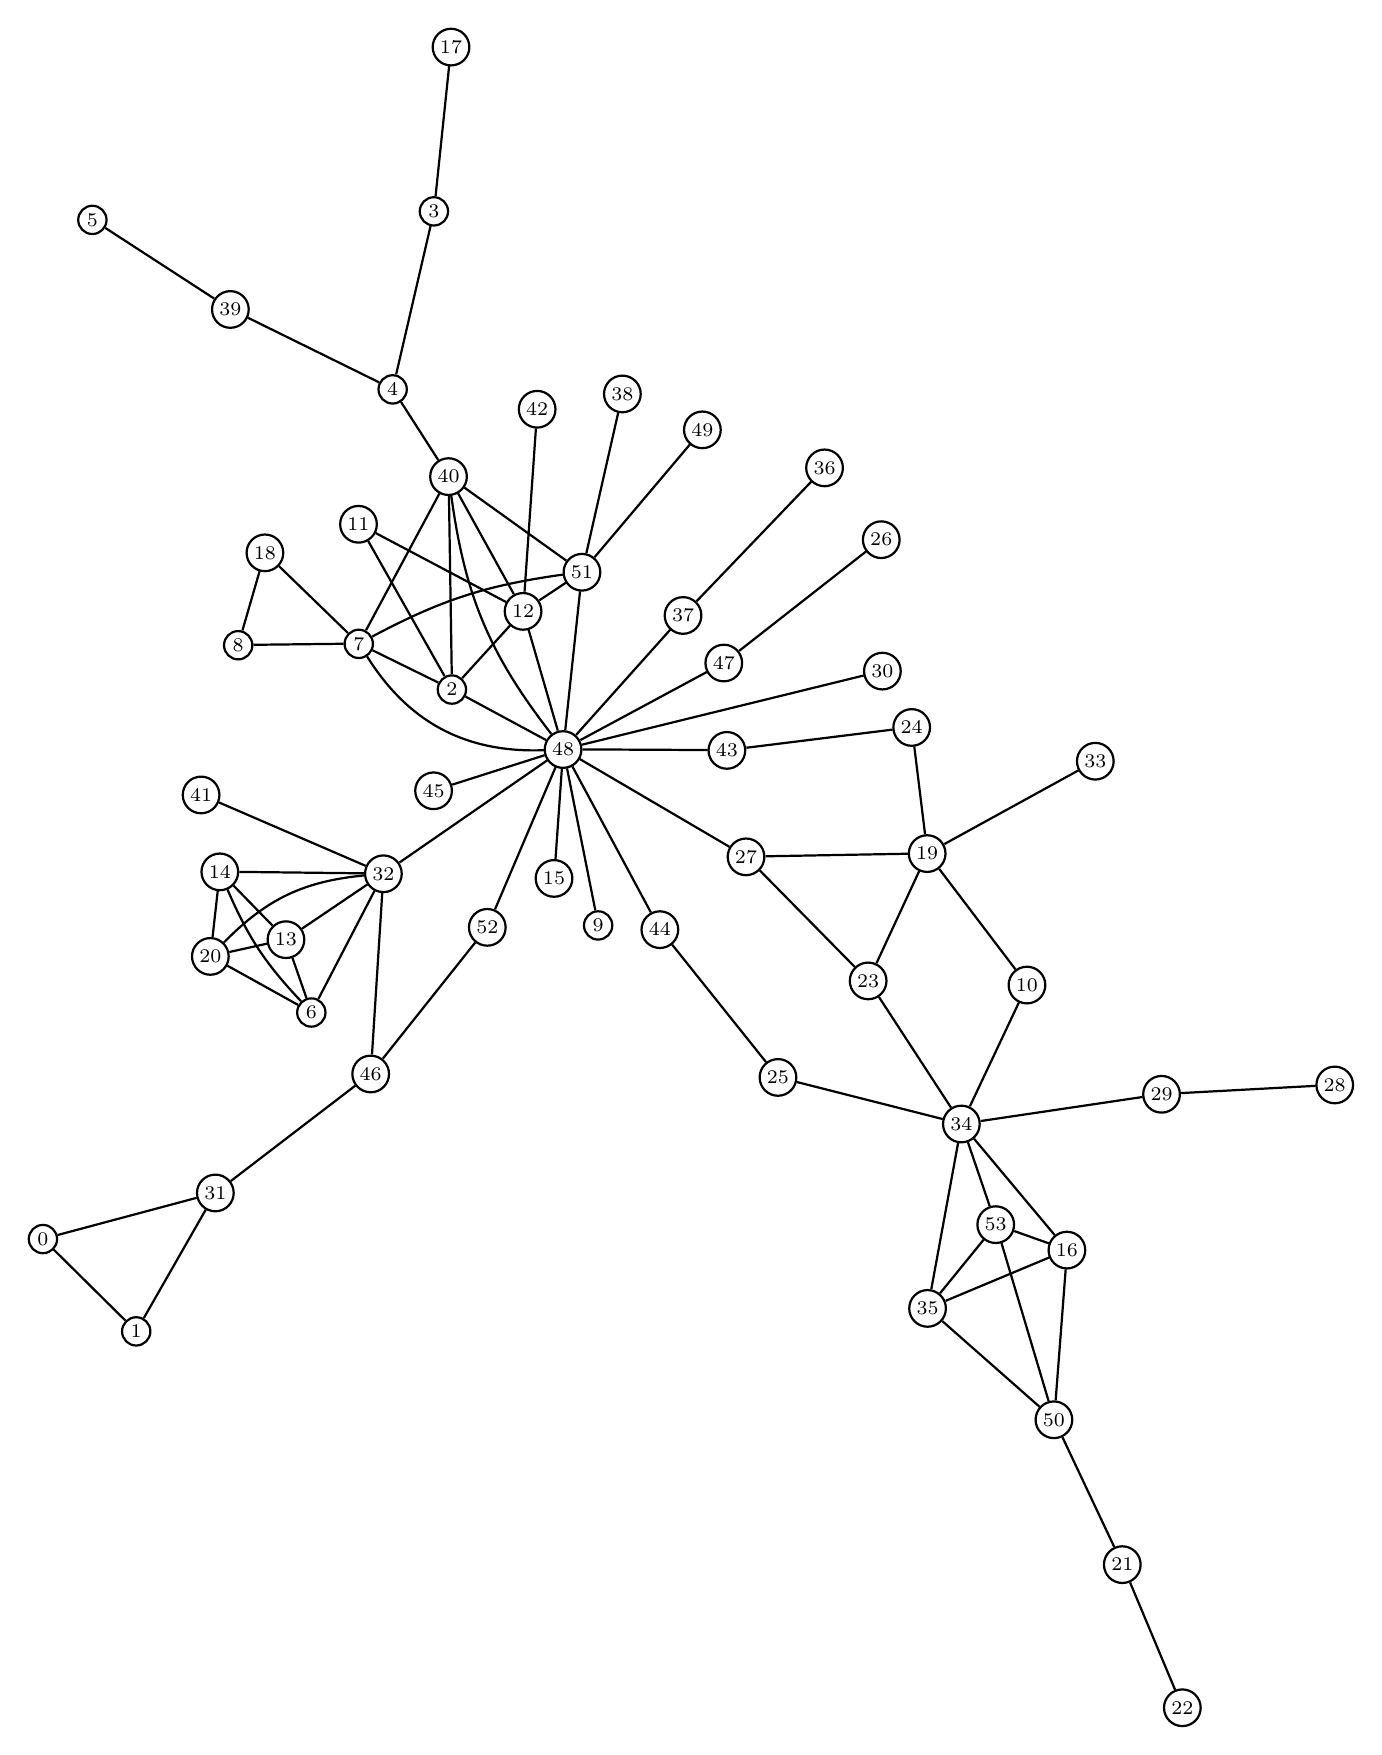
\begin{tikzpicture}
[lineDecorate/.style={-,thick},%
  nodeDecorate/.style={shape=circle,inner sep=1.5pt,draw,thick},%
  scale=1.9]
\scriptsize
%% nodes or vertices
\foreach \nodename/\x/\y in {
  0/0.38889/3.4037, 1/1.0124/2.7866, 2/3.1225/7.0766, 3/3.0023/10.273,
  4/2.7265/9.0831, 5/0.71937/10.216, 6/2.1829/4.918, 7/2.5/7.3821,
  8/1.694/7.3729, 9/4.1/5.5, 10/6.9664/5.1015, 11/2.4982/8.1814,
  12/3.5982/7.5993, 13/2.0133/5.4048, 14/1.5713/5.858, 15/3.8051/5.8142,
  16/7.2333/3.3299, 17/3.1167/11.371, 18/1.8727/7.9905, 19/6.2993/5.9802,
  20/1.5079/5.293, 21/7.6036/1.2275, 22/8.0049/0.27083, 23/5.9048/5.1292,
  24/6.1958/6.8233, 25/5.3021/4.4841, 26/5.9924/8.0784, 27/5.0885/5.9584,
  28/9.0236/4.4338, 29/7.8659/4.3714, 30/6/7.2, 31/1.5414/3.7119,
  32/2.6646/5.8454, 33/7.4232/6.5977, 34/6.5279/4.1727, 35/6.302/2.9402,
  36/5.6133/8.5584, 37/4.6675/7.5719, 38/4.262/9.0526, 39/1.6418/9.6172,
  40/3.1/8.5, 41/1.4461/6.3722, 42/3.6923/8.9503, 43/4.9606/6.6701,
  44/4.5126/5.4718, 45/3/6.4, 46/2.5796/4.5072, 47/4.9399/7.2539,
  48/3.8656/6.6757, 49/4.7967/8.8125, 50/7.1465/2.1958, 51/3.9918/7.8608,
  52/3.3592/5.4872, 53/6.7576/3.5}
{
  \node (\nodename) at (\x,\y) [nodeDecorate] {$\nodename$};
}
%% edges or lines
\path
\foreach \startnode/\endnode in {
  0/31, 0/1, 1/31, 2/48, 2/12, 2/11, 3/17, 3/4, 6/20, 6/13, 7/8,
  7/2, 7/40, 7/18, 8/18, 12/48, 12/11, 12/42, 13/20, 14/20, 14/13,
  16/34, 16/53, 19/10, 19/33, 19/24, 19/23, 19/27, 21/22, 27/23,
  27/48, 29/28, 32/41, 32/14, 32/13, 32/48, 32/6, 34/53, 34/10, 34/29,
  34/23, 34/25, 35/34, 35/53, 35/16, 37/48, 37/36, 39/4, 39/5, 40/4,
  40/12, 40/51, 40/2, 43/24, 43/48, 44/25, 44/48, 46/52,46/32, 46/31,
  47/26, 47/48, 48/9, 48/15, 48/45, 48/52, 48/30, 50/35, 50/16, 50/21,
  50/53, 51/12, 51/49, 51/38, 51/48}
{
  (\startnode) edge[lineDecorate] node {} (\endnode)
}
(6) edge[lineDecorate,bend left=10] node {} (14)
(7) edge[lineDecorate,bend right] node {} (48)
(7) edge[lineDecorate,bend left=10] node {} (51)
(20) edge[lineDecorate,bend left=20] node {} (32)
(40) edge[lineDecorate,bend right=15] node {} (48);
\end{tikzpicture}
\end{figure}

\end{document}

\caption{Network of common grape cultivars.}
\label{fig:distance_connectivity:wine_network}
\end{figure}

\item Figure~\ref{fig:distance_connectivity:wine_network} depicts how
  common grape\index{wine} cultivars are related to one another; the
  graph is adapted from Myles~et~al.~\cite{MylesEtAl2010}. The numeric
  code of each vertex can be interpreted according to
  Table~\ref{tab:distance_connectivity:wine_network}. Compute various
  distance and connectivity measures for the graph in
  Figure~\ref{fig:distance_connectivity:wine_network}.

\item Prove the characterizations of $2$-connected graphs as stated in
  Theorem~\ref{thm:distance_connectivity:characterization_2_connected_graphs}.

\item Let $G = (V,E)$ be an undirected connected graph of order $n$
  and suppose that $\deg(v) \geq (n + k - 2) / 2$ for all $v \in V$
  and some fixed positive integer $k$. Show that $G$ is
  $k$-connected.

\item A vertex~(or edge) separating set $S$ of a connected graph $G$
  is \emph{minimum} if $S$ has the smallest cardinality among all
  vertex~(respectively edge) separating sets in $G$. Similarly $S$ is
  said to be \emph{maximum} if it has the greatest cardinality among
  all vertex~(respectively edge) separating sets in $G$. For the graph
  in Figure~\ref{fig:separating_set:original_graph}, determine the
  following:
  %%
  \begin{enumerate}[(a)]
  \item A minimum vertex separating set.

  \item A minimum edge separating set.

  \item A maximum vertex separating set.

  \item A maximum edge separating set.

  \item The number of minimum vertex separating sets.

  \item The number of minimum edge separating sets.
  \end{enumerate}
\end{problem}
